\documentclass{article}
\setlength{\parskip}{0pt} % esp. entre parrafos
\setlength{\parindent}{20pt} % esp. al inicio de un parrafo
\usepackage{amsmath} % mates
\usepackage{listings}
\usepackage{xcolor}
\usepackage[sort&compress,numbers]{natbib} % referencias
\usepackage{url} % que las URLs se vean lindos
\usepackage[top=10mm,left=20mm,right=20mm,bottom=25mm]{geometry} % \textbf{\textbf{}}margenes
\usepackage{hyperref} % ligas de URLs
\usepackage{graphicx} % poner figuras
\usepackage{caption}
\usepackage{subcaption}
\usepackage[spanish]{babel} % otros idiomas
\hypersetup{
    colorlinks=true,
    linkcolor=blue,
    filecolor=blue,      
    urlcolor=blue,
}
\renewcommand{\lstlistingname}{Código}
\definecolor{codeblack}{rgb}{0,0.6,0}
\definecolor{codegray}{rgb}{0.5,0.5,0.5}
\definecolor{codepurple}{rgb}{0.58,0,0.82}
\definecolor{backcolour}{rgb}{0.95,0.95,0.92}
\lstdefinestyle{mystyle}{
    backgroundcolor=\color{backcolour},   
    commentstyle=\color{codeblack},
    keywordstyle=\color{blue},
    numberstyle=\tiny\color{codegray},
    stringstyle=\color{codeblack},
    basicstyle=\ttfamily\footnotesize,
    breakatwhitespace=false,         
    breaklines=true,                 
    keepspaces=true,                 
    numbers=left,                    
    numbersep=5pt,                  
    showspaces=false,                
    showstringspaces=false,
    showtabs=false,                  
    tabsize=2
}
\lstset{style=mystyle}

\title{"P12" Red neuronal}
\author{NESTOR}
\date {Mayo 2022}

\begin{document}

\maketitle

\section{Objetivo}\label{obj}
El objetivo de la práctica consiste en estudiar de manera sistemática el desempeño de la red neuronal en términos de su puntaje F (F-score en inglés) para los diez dígitos en función de las tres probabilidades asignadas a la generación de los dígitos (ngb), variando a las tres en un experimento factorial adecuado. \cite{elisa1}

\section{Desarrollo}\label{des}
Basando el desarrollo en la \href{https://github.com/satuelisa/Simulation/blob/master/NeuralNetwork/perceptron.py}{codificación} implementado por E. Schaeffer \cite{elisa1} y todas las instrucciones se encuentra en el \href{https://github.com/NestorZeus/SIMULACION-COMPUTACIONAL-DE-NANOMATERIALES/tree/main/P12}{repositorio} de N. Rodríguez en GitHub.\\

Para comenzar se hace la función factorial para los modelos de las probabilidades negro, gris y blanco al número que se ingreso.

\begin{lstlisting}[caption=Generamos la función, language=Python]
import itertools
from math import floor, log
import pandas as pd
factorial= itertools.product((1,0.5,0),(1,0.5,0),(1,0.5,0))
resultados=[]
for d1, d2, d3 in factorial:
    print('##############',d1,d2,d3,'###############')
    ciclos=10
    Rpl=[]
    for rpt in range(ciclos):
        modelos = pd.read_csv('digits.txt', sep=' ', header = None)
        modelos = modelos.replace({'n': d1, 'g': d2, 'b': d3})
\end{lstlisting}

Posteriormente se genera el F-score haciendo que se genere la matriz en confusión con la $c$ 

\begin{lstlisting}[caption=Generamos F-score, label=codigo2, language=Python]
c = pd.DataFrame(contadores)
c.columns = [str(i) for i in range(k)] + ['NA']
c.index = [str(i) for i in range(k)]
        arr=c.to_numpy()
        TP=sum(arr.diagonal())
        FP=(sum(sum(arr[:,:tope])))-TP
        FN= sum(sum(arr[:,-1:]))
        Precision= TP/(TP+FP)
        Recuperacion= TP/(TP+FN)
        puntajeF= 2*(Precision*Recuperacion)/(Precision+Recuperacion)
        Rpl.append(puntajeF)
resultados.append(Rpl)
\end{lstlisting}

\section{Resultados}\label{res}
Se visualiza para la primer combinación ($1$, $1$, $1$) fue un F-score aproximado de $0.2$, aquí lo que se busca es tener el F-score muy alto porqué se reconoció cai todos los números. ya que todas las combinaciones de las probabilidades se variaron y se hicieron réplicas y esas réplicas de ($1$, $0.5$, $0.5$) y ($0$, $0.5$, $0.5$) se obtuvo el cien porciento de número de detección correcta de verdaderos positivos un F-score alto. 

\begin{figure}
    \centering
    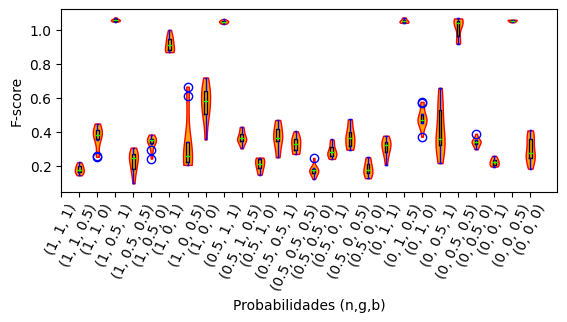
\includegraphics[width=150mm]{Figure_1.png}
    \caption{Diagrama de F-score}
    \label{figure}
\end{figure}


\section{Conclusiones}\label{}
Vimos un mejor comportamiento de F-score para las combinaciones ($1$, $1$, $0$), ($1$, $0.5$, $0.5$), ($0$, $0.5$, $0.5$), ($0.5$, $1$, $1$), ($0$, $1$, $0.5$) y ($0$, $0$, $0.5$) esto es un F-score muy alto.


\newpage
\section{Reto 1 Red neuronal con símbolos ASCII }\label{}
En este reto consiste en la red neuronal para que reconozca además por lo menos doce símbolos ASCII adicionales, aumentando la resolución de las imágenes a $5$ x $7$ de lo original de $3$ x $5$ (modificando las plantillas de los dígitos acorde a este cambio).

\begin{lstlisting}[caption=Se hace la modificación de modelos de $7$ y $5$, language=Python]
modelos = pd.read_csv('digits_12.txt', sep=' ', header = None)
modelos = modelos.replace({'n': d1, 'g': d2, 'b': d3})
r, c = 7, 5
dim = r * c
tasa = 0.15
tranqui = 0.99
tope = 21
\end{lstlisting}


\section{Reto 1 Resultados}\label{}
Se extendió la librería de reconocimiento de dígitos con $12$ símbolos más y esta es la imagen de $5$ x $7$ mismo código.

\begin{figure}
    \centering
    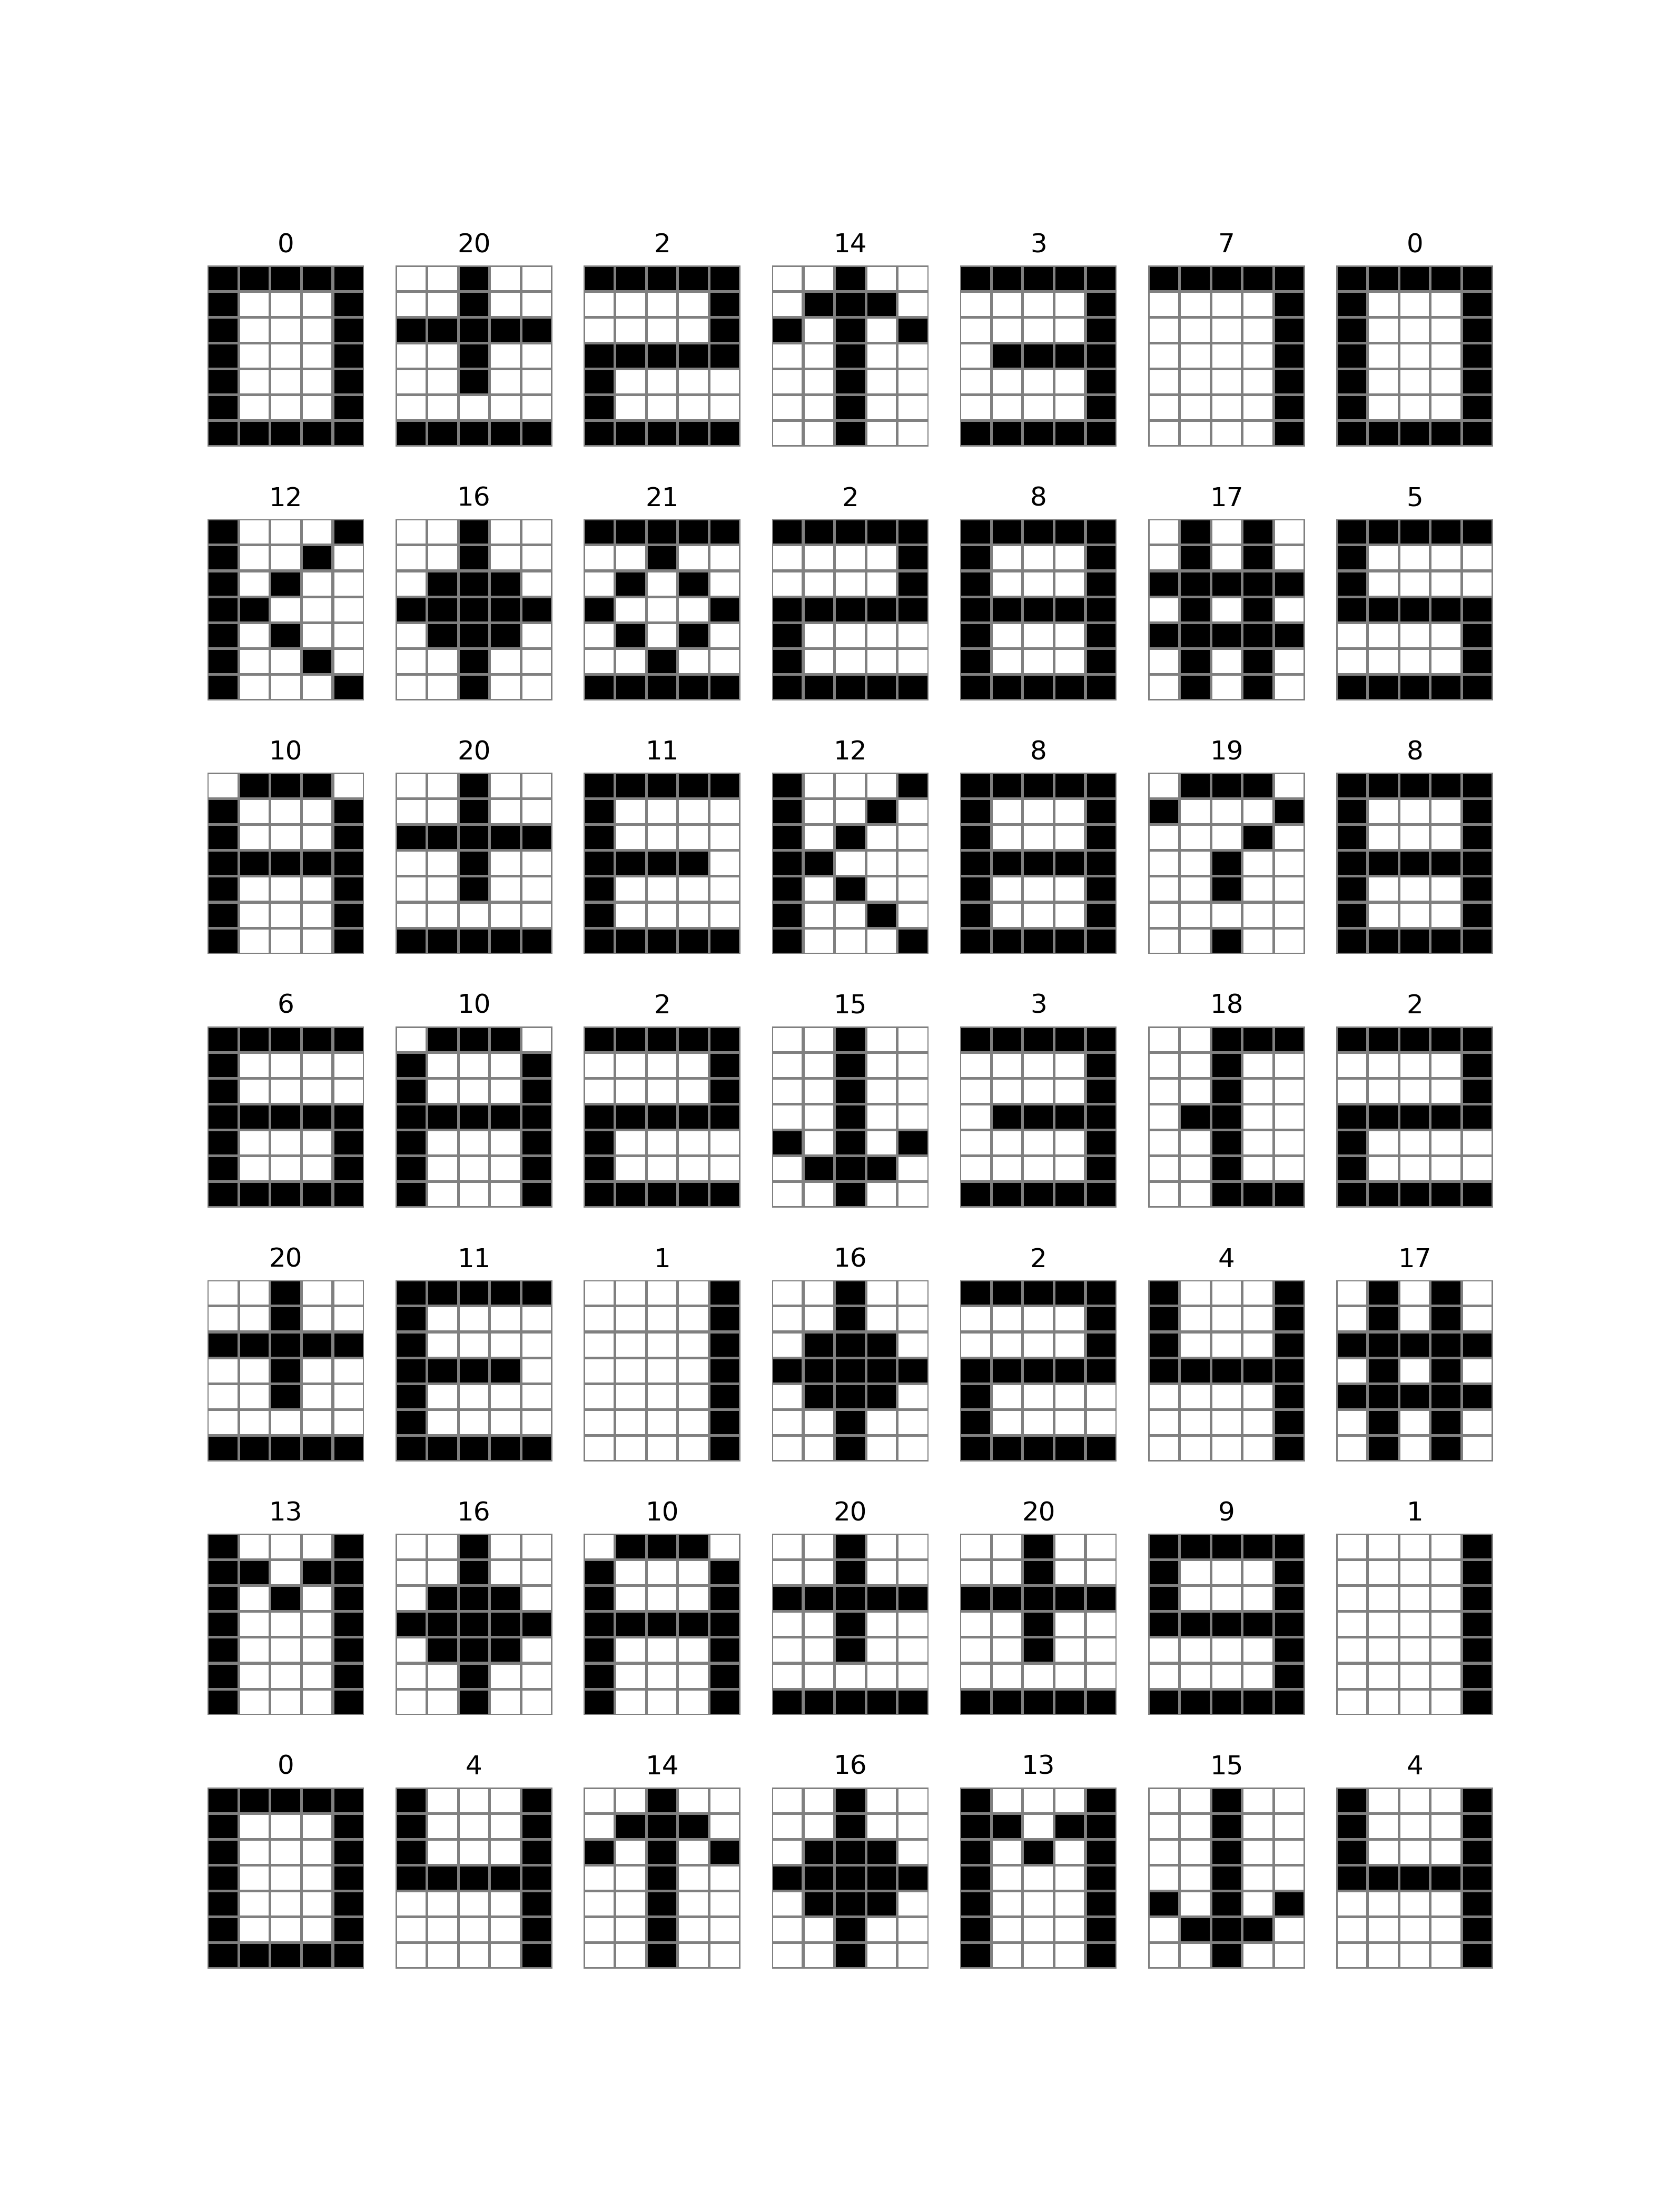
\includegraphics[width=190mm]{Figure_3.png}
    \caption{Diagrama de símbolos ASCII}
    \label{figure}
\end{figure}

\newpage

\section{Reto 2 Se estudia el ruido sal y pimienta}\label{}
En este reto consiste en las entradas para una combinación ngb con la cual la red desempeña bien; este tipo de ruido se genera cambiando con una probabilidad $pr$ los pixeles a blanco o negro (uniformemente al azar entre las dos opciones).

\begin{lstlisting}[caption=Se fijan los valores con el mismo ciclo, language=Python]
for pr in (0.1,0.2,0.3,0.4,0.5,0.6,0.7,0.8,0.9,1):
    print('##############',pr,'###############')
    ciclos=10
    Rpl=[]
    for rpt in range(ciclos):
        modelos = pd.read_csv('digits.txt', sep=' ', header = None)
        modelos = modelos.replace({'n': 1, 'g': 0, 'b': 0})
        r, c = 5, 3
        dim = r * c
        tasa = 0.15
        tranqui = 0.99
        tope = 9
\end{lstlisting}

Para este de la fase de entrenamiento aquí está el cambio de sal y pimienta.
\begin{lstlisting}[caption=Fijamos los valores, language=Python]
for t in range(5000): # entrenamiento
    d = randint(0, tope)
    pixeles = 1 * (np.random.rand(dim) < modelos.iloc[d])
    if (random.uniform(0, 1)) < pr:
        pixeles= random.randint(0, 1)* np.random.rand(dim)
for t in range(300): # prueba
    d = randint(0, tope)
    pixeles = 1 * (np.random.rand(dim) < modelos.iloc[d])
    if (random.uniform(0, 1)) < pr:
        pixeles= random.randint(0, 1)* np.random.rand(dim)
\end{lstlisting}

\section{Reto 2 Resultados}\label{}
Se muestra resultados de agresor ruido sal y pimienta son cuando la probabilidad es muy baja casi no se modifica la imagen y por lo tanto F-score sale alto ya que hubo muy buena detección de muchos verdaderos positivos en la matriz. 

\begin{figure}
    \centering
    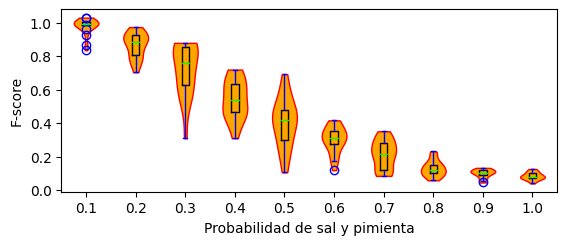
\includegraphics[width=195mm]{Figure_4.png}
    \caption{Diagrama de sal y pimienta.}
    \label{figure}
\end{figure}

\newpage
\bibliographystyle{plainnat}
\bibliography{simulacion}
\end{document}
